\documentclass[t]{beamer}
\usepackage[utf8]{inputenc}  % to be able to type unicode text directly
%\usepackage[french]{babel}   % french typographical conventions
\usepackage{inconsolata}     % for a nicer (e.g. non-courier) tt family font
\usepackage{amsthm,amsmath}  % fancier mathematics
\usepackage{mathabx}         % even fancier mathematics
\usepackage{array}           % to fine-tune tabular spacing
\usepackage{bbm}             % for blackboard 1
\usepackage{textpos}         % absolute positioning
\usepackage{hyperref,url}    % links and urls

\usepackage{graphicx}        % to include images
%\usepackage{animate}         % to include animated images
%\usepackage{bbding}          % for Checkmark and XSolidBrush
%\usepackage[outputdir=PDFLATEXFILTERD]{minted}          % for code insets
\usepackage{minted}          % for code insets
\usepackage{soul}            % for colored strikethrough

\colorlet{darkgreen}{black!50!green}  % used for page numbers
\definecolor{term}{rgb}{.9,.9,.9}     % used for code insets

\setlength{\parindent}{0em}
\setlength{\parskip}{1em}


% coco's macros
\newcommand{\1}{\textbf{1}}
\def\R{\textbf{R}}
\def\C{\textbf{C}}
\def\N{\textbf{N}}
\def\T{\textbf{T}}
\def\F{\mathcal{F}}
\def\x{\textbf{x}}
\def\y{\textbf{y}}
\def\b{\textbf{b}}
\def\u{\mathbf{u}}
\def\Z{\textbf{Z}}
\def\d{\mathrm{d}}
\DeclareMathOperator*{\argmin}{arg\,min}
\DeclareMathOperator*{\argmax}{arg\,max}
\newcommand{\reference}[1] {{\scriptsize \color{gray}  #1 }}
\newcommand{\referencep}[1] {{\tiny \color{gray}  #1 }}
\newcommand{\unit}[1] {{\tiny \color{gray}  #1 }}

% \parens{x}      ->  (x)
% \pairing{x}{y}  ->  <x,y>
\newcommand{\parens}[1]{\left(#1\right)} % (x)
\newcommand{\pairing}[2]{\left\langle #1,\,#2\right\rangle} % <x,y>

% \abs{x}         ->    |x|
% \Abs{x}         ->   ||x||
% \ABS{x}         ->  |||x|||
\newcommand{\abs}[1]{\left|#1\right|}
\newcommand{\Abs}[1]{\left\|#1\right\|}
\newcommand{\ABS}[1]{{\left\vert\kern-0.25ex\left\vert\kern-0.25ex\left\vert #1 \right\vert\kern-0.25ex\right\vert\kern-0.25ex\right\vert}}

% \Sh -> dirac comb symbol shah
\DeclareFontFamily{U}{wncy}{}
\DeclareFontShape{U}{wncy}{m}{n}{<->wncyr10}{}
\DeclareSymbolFont{mcy}{U}{wncy}{m}{n}
\DeclareMathSymbol{\Sh}{\mathord}{mcy}{"58}

% really wide hat
\usepackage{scalerel,stackengine}
\stackMath
\newcommand\reallywidehat[1]{%
\savestack{\tmpbox}{\stretchto{%
  \scaleto{%
    \scalerel*[\widthof{\ensuremath{#1}}]{\kern-.6pt\bigwedge\kern-.6pt}%
    {\rule[-\textheight/2]{1ex}{\textheight}}%WIDTH-LIMITED BIG WEDGE
  }{\textheight}% 
}{0.5ex}}%
\stackon[1pt]{#1}{\tmpbox}%
}

% disable spacing around verbatim
\usepackage{etoolbox}
\makeatletter\preto{\@verbatim}{\topsep=0pt \partopsep=0pt }\makeatother

% disable headings, set slide numbers in green
\mode<all>\setbeamertemplate{navigation symbols}{}
\defbeamertemplate*{footline}{pagecount}{\leavevmode\hfill\color{darkgreen}
   \insertframenumber{} / \inserttotalframenumber\hspace*{2ex}\vskip0pt}

%%% select red color for strikethrough
\makeatletter
\newcommand\SoulColor{%
  \let\set@color\beamerorig@set@color
  \let\reset@color\beamerorig@reset@color}
\makeatother
\newcommand<>{\St}[1]{\only#2{\SoulColor\st{#1}}}
\setstcolor{red}

% make everything monospace
\renewcommand*\familydefault{\ttdefault}

\begin{document}

\addtocounter{framenumber}{-1}
\begin{frame}[plain,fragile]
\LARGE
\begin{verbatim}




    ipol.sh  and  ipol.py





EML
GTTI 9--12--2020
\end{verbatim}
\end{frame}


\begin{frame}[fragile]
IPOL.PY AND IPOL.SH\\
===================

{\bf What:}\\
{\color{blue}Natural} shell and python interfaces for many IPOL algorithms.

{\bf How:}\\
A single file {\color{blue}ipol.py} that can be imported from Python or run
from the command line.

{\bf Why:}\\
\pause
{\St{To troll Miguel.}}$ $
For various serious reasons.

\vfill
\pause
{\bf Status:}\\
%- {\color{blue}github.com/mnhrdt/clipol}\\
%- {\color{blue}git.sr.ht/\verb+~+coco/clipol}\\
- {\color{blue}\url{git.sr.ht/~coco/clipol}}\\
- Works on Linux, BSDs and macOS Catalina, no Windows\\
- Missing support for octave/torch/tensorflow\\
- Must add ``all'' IPOL algorithms (only 10 yet)
\end{frame}


% THE WHAT
\begin{frame}%

\vfill
\begin{center}
\Huge
The \bf What
\end{center}
\vfill
\small
{$\,$ {\bf Natural interfaces} to IPOL algorithms in shell and Python}
\end{frame}

% what is a ``natural'' interface for LSD in shell and python
% (natural frontend)
\begin{frame}[fragile]
NATURAL PYTHON AND SHELL INTERFACES FOR LSD\\
===========================================

\vfill
{\bf ``Natural''} way to run LSD inside Python:
\begin{minted}[frame=single]{python}
import ipol       # the proposed interface to IPOL
x = ...           # create an image as an ndarray
y = ipol.lsd(x)   # y is now an array of size Nx7
\end{minted}


\vfill
{\bf ``Natural''} way to run LSD inside the shell:
\begin{minted}[frame=single]{bash}
ipol lsd image.png segments.txt
\end{minted}

\vfill
\end{frame}

% ease to concatenate demos: e.g. ponomarenko+denoising
\begin{frame}[fragile]
CONCATENATION OF IPOL ALGORITHMS\\
================================

{\bf Goal:}
Estimate the noise of an image using Ponomarenko's method, then denoise it
using NLM.

\vfill
In Python:
\begin{minted}[frame=single]{python}
import ipol, iio
x = iio.read("barbara.png")
s = ipol.ponomarenko(x)
y = ipol.nlm(x, s)
iio.write("barbara_denoised.png")
\end{minted}

\vfill
In the shell:
\begin{minted}[frame=single]{bash}
S=`ipol ponomarenko barbara.png -`
ipol nlm sigma=$S barbara.png barbara_denoised.png
\end{minted}

\end{frame}

% python help (with completion)
\begin{frame}[fragile]
PYTHON HELP VIA COMPLETION\\
==========================

Typing
\begin{minted}[frame=single]{python}
import ipol

ipol.scb(
\end{minted}
inside a modern interface shows the auto-generated help message for the
algorithm "scb":
\begin{minted}[frame=single]{python}
# Simplest Color Balance
# out = scb(in, Smin=1, Smax=1, mode="rgb")
\end{minted}

\end{frame}

% shell help (with completion)
\begin{frame}[fragile]
SHELL HELP OPTION\\
=================

Similarly, typing
\begin{minted}[frame=single]{shell}
ipol scb
\end{minted}
on the shell gives the help for that sub-command
\footnotesize
\begin{minted}[frame=single]{shell}
Simplest Color Balance
Usage:
        ipol scb in.png [Smin=1] [Smax=1] [mode="rgb"] out.png
\end{minted}
\end{frame}

% frontend design criteria
\begin{frame}
EXISTING ALGORITHMS\\
===================

Some IPOL algorithms have already been adapted to this system:
{\color{blue}
lsd, tvl1flow, phsflow, roflow, rdpoflow, ace, %bm3d,
sift, asift,
goldstein-fattal, canny-devernay, retinex-poisson, nlm, dct-denoise
}

The adaptation consists in reading and understanding the README file of the
code, and call it from the command line.  Equivalent to writing the
{\color{blue} run.sh} file in the demo system.  Estimated time per
algorithm:~{\bf 15min}.
\end{frame}

% frontend design criteria
\begin{frame}
FRONTEND DESIGN CRITERIA\\
========================

1. Each algorithm has a
{\color{blue}unique},
{\color{blue}meaningful
%well-chosen
name}.

2. The interface is as natural as possible, and selects {\color{blue}reasonable
defaults} for missing parameters.

3. Raw access to the original executable is available via the option
{\color{blue}--raw}.

4. Transparent conversion to the image format chosen by each program.  The
default file format is {\color{blue}.npy}.
\end{frame}

% ``natural'' bakend: idl
\begin{frame}[fragile]
BACKEND: IDL FILES (INSPIRED BY DOCKERFILES)\\
============================================

Complete {\bf IDL} file for LSD:

\begin{minted}[frame=single,fontsize=\small]{docker}
NAME lsd
TITLE Line Segment Detector
SRC http://www.ipol.im/pub/art/2012/gjmr-lsd/lsd_1.6.zip

INPUT in image pgm
OUTPUT out image

BUILD make
BUILD cp lsd $BIN

RUN lsd $in $out
\end{minted}
\end{frame}

\begin{frame}[fragile]
BACKEND: IDL FILES (INSPIRED BY DOCKERFILES)\\
============================================

Complete {\bf IDL} file for LSD:

\begin{minted}[frame=single,fontsize=\small]{docker}
NAME lsd  # global identifier
TITLE Line Segment Detector
SRC http://www.ipol.im/pub/art/2012/gjmr-lsd/lsd_1.6.zip

INPUT in image pgm  # the input image is converted to pgm
OUTPUT out image

BUILD make          # shell instructions to build the program
BUILD cp lsd $BIN   # program files are copied to $BIN

RUN lsd $in $out    # $BIN is in the path, you can run lsd
\end{minted}
Comments are allowed!
\end{frame}

% a more complex idl with per-uname differences
\begin{frame}[fragile]
A MORE COMPLEX IDL FILE\\
=======================

\begin{minted}[frame=single,fontsize=\footnotesize]{docker}
NAME    scb
TITLE   Simplest Color Balance
AUTHORS N.Limare, J.-L.Lisani, J.-M.Morel, A.Belén Petro, C.Sbert
SRC     http://www.ipol.im/pub/art/2011/llmps-scb/simplest_color_balance.tar.gz

BUILD   make
BUILD   cp balance $BIN/scb

INPUT   in    image
INPUT   Smin  number 1      # percentage saturated to min
INPUT   Smax  number 1      # percentage saturated to max
INPUT   mode  string rgb    # rgb or irgb
OUTPUT  out   image

RUN     scb $mode $Smin $Smax $in $out
\end{minted}
\color{red}{\bf Note:}
This was written after a fast read of the code's README file
\end{frame}

\begin{frame}[fragile]
A MORE COMPLEX IDL FILE\\
=======================

\begin{minted}[frame=single,fontsize=\footnotesize]{docker}
NAME    tvl1flow
TITLE   TVL1 Optical Flow
SRC     http://www.ipol.im/pub/art/2013/26/tvl1flow_3.tar.gz

BUILD   make
BUILD   cp tvl1flow $BIN

INPUT   a   image png
INPUT   b   image png
OUTPUT  out image flo

RUN     tvl1flow $a $b $out
\end{minted}
%BUILD:OpenBSD make CC="cc -std=c99" OMPFLAGS="-DDISABLE_OMP"
%BUILD:OpenBSD cp tvl1flow $BIN

\color{red}{\bf Note:}
The actual file has several optional parameters
\end{frame}

\begin{frame}[fragile]
IDL SPECIFICATION {\color{red}(for rafa)}\\
============================

\begin{minted}[frame=single,fontsize=\footnotesize]{docker}
An IDL file is a sequence of lines of text.

Each line is of the form "COMMAND option1 option2 ...".

There are 7 commands: NAME TITLE SRC INPUT OUTPUT BUILD RUN

There will never be more than these commands, and
"TITLE" may be removed in the future, or replaced by "DOC".
You can add user-readable text by using #-comments.

NAME <id>                             # how to call the algorithm
TITLE <unquoted-string-max-68-chars>  # title of the article
SRC <url>                             # where to get the source code
BUILD <command-line>                  # build instructions
INPUT <id> <type>                     # obligatory input argument
INPUT <id> <type> <default-value>     # optional input argument
OUTPUT <id> <type>                    # obligatory output argument
OUTPUT <id> <type> optional           # optional output argument
RUN <command-line>                    # run instructions
\end{minted}

\end{frame}

% list of current IDL files
%\begin{frame}
%EXISTING IDL FILES\\
%==================
%
%\end{frame}


\begin{frame}
OPEN DESIGN PROBLEM NUMBER 1\\
============================

Single namespace or submodules?

{\color{blue}$\qquad$ ipol.tvl1flow}

vs.

{\color{blue}$\qquad$ ipol.of.tvl1}

\end{frame}

\begin{frame}[fragile]\small
OPEN DESIGN PROBLEM NUMBER 2\\
============================

What format for IDL files: "docker" vs "ini"?
% put an .ini file here
\vspace{-1em}
\begin{minted}[frame=single,fontsize=\scriptsize]{bash}
[info]
name = ace
longname = Automatic Color Enhancement
authors = Pascal Getreuer
src = http://www.ipol.im/pub/art/2012/g-ace/ace_20121029.tar.gz

[input]
in = image
alpha = number : 5
omega = string : 1/r
method = string : interp5

[output]
out = image

[build]
make -f makefile.gcc
cp ace $BIN

[run]
ace -a $alpha -w $omega -m $method $in $out
\end{minted}
\end{frame}

\begin{frame}[fragile]\small
OPEN DESIGN PROBLEM NUMBER 2\\
============================

What format for IDL files: "docker" vs "ini"?
% put an .ini file here
\vspace{-1em}
\begin{minted}[frame=single,fontsize=\scriptsize]{docker}
NAME    ace
TITLE   Automatic Color Enhancement
AUTHOR  Pascal Getreuer
SRC     http://www.ipol.im/pub/art/2012/g-ace/ace_20121029.tar.gz

BUILD   make -f makefile.gcc
BUILD   cp ace $BIN

INPUT   image   in
INPUT   number  alpha   5
INPUT   string  omega   1/r
INPUT   string  method  interp5

OUTPUT  image   out

RUN     ace -a $alpha -w $omega -m $method $in $out
\end{minted}
\end{frame}

\begin{frame}[fragile]\small
OPEN DESIGN PROBLEM NUMBER 2\\
============================

What format for IDL files: "docker" vs "ini"?
% put an .ini file here
\vspace{-1em}
\begin{minted}[frame=single,fontsize=\scriptsize]{docker}
NAME    ace
TITLE   Automatic Color Enhancement
AUTHOR  Pascal Getreuer
SRC     http://www.ipol.im/pub/art/2012/g-ace/ace_20121029.tar.gz

BUILD   make -f makefile.gcc
BUILD   cp ace $BIN

INPUT   in      image
INPUT   alpha   number  5
INPUT   omega   string  1/r
INPUT   method  string  interp5

OUTPUT  out     image

RUN     ace -a $alpha -w $omega -m $method $in $out
\end{minted}
\end{frame}


% THE HOW
\begin{frame}%

\vfill
\begin{center}
\Huge
The \bf How
\end{center}
\vfill
\small
\centering
{A single file {\bf ipol.py}}
\end{frame}


% how does it work, what does it do internally?
\begin{frame}
INNER WORKINGS OF ipol.py\\
=========================

1. A single file {\color{blue}ipol.py} that you can\\
import (from Python) or run (from the shell)

2. The first call to {\color{blue}ipol.X()} downloads and compiles the source
code into {\color{blue}\url{~/.cache/ipol/X/bin}}

3. Subsequent calls reuse this pre-compiled code

4. A local archive of all computed inputs/outputs is kept on
{\color{blue}\url{~/.cache/ipol/X/archive}}

5. Idl files are kept in {\color{blue}\url{~/.config/ipol/idl}}

\end{frame}

\begin{frame}[fragile]
FUNNY IMPLEMENTATION DETAILS\\
============================

How to generate functions from a string:
\begin{minted}[fontsize=\scriptsize]{python}
def export_article_interface(x):
        __import__("ipol").__dict__[x] = lambda *a, **k : run_article(x, a, k)
\end{minted}

\pause
Then you can do:
\begin{minted}[fontsize=\scriptsize]{python}
export_article_interface("scb")    # create a global function named ipol.scb
y = ipol.scb(x, Smin=2, Smax=2)    # call run_article("scb", x, ...)
\end{minted}

\vfill
\pause
And, to generate the docstrings:
\begin{minted}[fontsize=\scriptsize]{python}
globals()["scb"].__doc__ = ...
\end{minted}


\end{frame}

% the inner working is an implementation detail
% comment: enforcing stricter software guidelines would make an easier, more
% efficient integration trivial
%\begin{frame}
%IPOL.PY AND IPOL.SH\\
%===================
%
%\end{frame}


% THE WHY
\begin{frame}%

\vfill
\begin{center}
\Huge
The \bf Why
\end{center}
\vfill
\small
\centering
{Various serious reasons}
\end{frame}

%\begin{frame}
%$\!\,${\bf WHY:} SUMMARY OF REASONS\\
%=======================
%
%1. Proof-based reproducibility\\
%(as opposed to trust-based for ipol demos)
%
%2. Personal usage: avoid re-reading the README file every time I want to run an
%ipol code.
%
%3. Personal challenge: write a sane Python program
%
%4. Towards a ``corpus'' of algorithms like in megawave
%
%\end{frame}

% trust-based reproducibility in current ipol demos
% goal: proof-based reproducibility
\begin{frame}
$\!\,$REASON NUMBER 1: {\bf\color{darkgreen}PROOF}-BASED REPRODUCTIBILITY\\
==============================================

Reproductibility offered by IPOL demos entails a certain level of
{\color{red}trust}: you see that the authors can produce the results, but are
they really using the published algorithm?  Are there hidden parameters inside
{\color{red}run.sh}?

\pause
The only way to be sure is to download and
{\bf \color{darkgreen}run the code locally}!

\end{frame}


% in more practical terms: avoid reading the ''README'' for each new ipol code
% we want to try.  The IDL formalizes (and thus replaces) the README file
\begin{frame}
REASON NUMBER 2: FORMALIZATION OF THE README FILE
=================================================

To use a new IPOL code, we have to read and understand the provided README
file, which is a {\color{red}freely-formatted text},
with {\color{red}different conventions} for each
article.

The IDL files serve as a formalization of the various READMEs.  Thus, they are
a {\bf\color{darkgreen} formal documentation} that is useful in itself (even if
you don't use ipol.py).

\end{frame}

\begin{frame}
REASON NUMBER 3: ANSWERS A PRACTICAL NEED\\
=========================================

Charles' python bindings to IPOL algorithms, for example
{\color{blue}\url{github.com/cmla/ponomarenko}}:

{\color{red}
- a whole git repository\\
- seven particular files\\
- in-place Makefile tweaks\\
- ad-hoc pipy integration\\
- 3 months-long development\\
}{\bf\color{darkgreen}- fast, in-memory, zero-overhead interface}

\vfill
Similar repos:

{\color{blue}\url{github.com/cmla/{ransac,plyflatten,sift,srtm4}}}:\\
several ad-hoc python bindings to C+shell algorithms
\end{frame}

\begin{frame}
	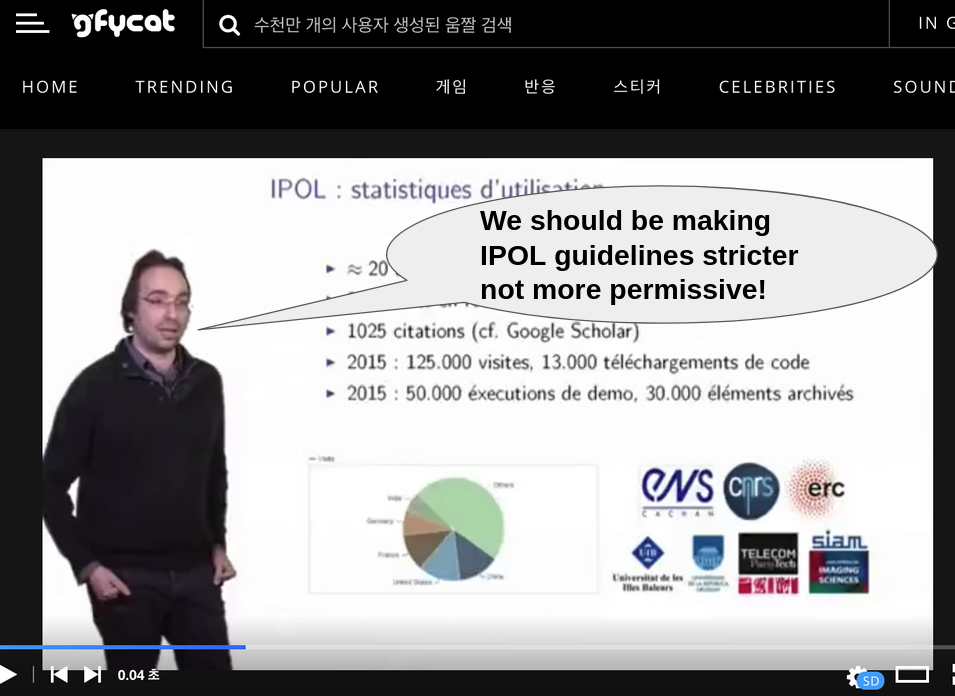
\includegraphics[height=\textheight]{f/shittycoco.png}
\end{frame}

% personally, a proof of sane python coding style
% - indentation with tabs
% - all variables are single letters
% - no global imports
% - no bullshit like json, pandas, and the like
\begin{frame}
REASON NUMBER 4: PERSONAL GROWTH\\
================================

This is my "first" Python program, I had great fun learning it.

\pause
Also, I used a (non-standard) {\bf\color{darkgreen}sane
Python coding style}:

- all code in a single file\\
- no global imports\\
- no classes\\
- no exceptions\\
- no bullshit like json, pandas, and the like\\
- all local variables are single letters\\
- all strings are f-strings, no .format\\
- indentation with tabs\\
- non PEP-8 compliant\\

\end{frame}


% build a corpus of algorithm à la megawave that are runnable and comparable
% together.  Goal: never get to ``de-ipolisize'' a code in the future.
\begin{frame}[fragile]
REASON NUMBER 5: STABILIZE THE CORPUS OF ALGORITHMS\\
===================================================

In the olden days we had everything on {\color{blue}Megawave}.
Now, to use megawave codes we have to un-megawaveize them.

I hope that we'll never have to un-ipolize a code!

\vfill
\pause
{\bf Relistic example} from the "ace" description file:
\begin{minted}[frame=single,fontsize=\scriptsize]{docker}
# general build instructions
BUILD make -f makefile.gcc
BUILD cp ace $BIN

# build instructions for systems whose "uname" matches OpenBSD
BUILD:OpenBSD sed -i~ 85d acecli.c      # delete openmp line
BUILD:OpenBSD sed -i~ 1317d imageio.c   # delete openmp line
BUILD:OpenBSD gmake -f makefile.gcc OPENMP="" CFLAGS="-std=c99 -O3"
BUILD:OpenBSD cp ace $BIN
\end{minted}
\vfill
\end{frame}


% design phylosopy (from more important to less important)
% 1. Super-simple shell interface
% 2. Super-simple Python interface
% 3. Super-simple IDL files (goal: write a new IDL file in less than 15min)
% 4. Minimum number of Python dependencies
% 5. Super-simple Python implementation
% 6. Portability to as many IPOL algorithms as possible
% 7. Portability to as many systems as possible
% 8. Efficient runtime
\begin{frame}
DESIGN PHILOSOPHY\\
=================

From more to less important:

0. Offer proof-based reproductibility\\
1. Super-simple shell interface\\
2. Super-simple Python interface\\
3. Super-simple IDL files (goal: 1 IDL file $\le$ 15min)\\
4. Minimum number of Python dependencies\\
5. Super-simple Python implementation\\
6. Portability to as many IPOL algorithms as possible\\
7. Portability to as many systems as possible\\
8. Efficient runtime\\

\end{frame}

% status and future work
\begin{frame}
STATUS AND FUTURE WORK\\
======================

{\bf ipol.py:}\\
A {\color{darkgreen}natural} and
{\color{darkgreen}local} python+shell interface to IPOL

{\bf Status:}\\
{\color{darkgreen}Exists},
{\color{red}clunky implementation},
{\color{red}has many bugs},
{\color{red}not~well-documented},
{\color{red}not~feature-complete}

{\bf Future work:}\\
write lots of IDL files,
fix bugs,
{\color{blue}pip install ipol},
\\
improve autogenerated docstrings,\\
adapt to trained torch/tf models

{\bf Far future:}\\
auto-generated efficient C interfaces by adding a CFFI command to the IDL files

\pause
{\bf Trolling:}
add {\color{blue}--serve-http} option


\end{frame}

% support promise: 1 idl file = 1 pint of beer (of my choice)
\begin{frame}
PUBLICITY\\
=========

Do you think it can be useful for you?

No need to learn to write IDL files!

I offer support at the price of

\color{blue}
\fbox{
\fbox{
\fbox{
\fbox{1 IDL file = 1 pint of beer (of my choice)}
}}}

\end{frame}

\end{document}


% vim:sw=2 ts=2 spell spelllang=fr:
